\subsection{Models}

To assess the impact of DP mechanisms on the performance and interpretability of AD models, we develop a sequence of progressively privatized autoencoder models. These models serve as the core components of our experimental framework, enabling a fair and controlled comparisons across varying levels of privacy intervention. Each model builds upon a shared architectural foundation, which is autoencoder, but differs in the stage and manner in which privacy is introduced, ranging from fully non-private training to DP-SGD optimization and post-hoc output perturbation. Following model construction and accuracy evaluation, we apply XAI techniques to each variant to examine how the introduction of privacy affects the interpretability of model decisions. 

\subsubsection{Baseline Autoencoders} \label{s:method_baseline}

To establish a reference point for evaluating the effects of DP mechanisms, we first implement a standard non-private autoencoder model as a benchmark. This baseline model is trained on a subset of the data that contains only normal samples, following conventional procedures as described in Section~\ref{s:background_ae}. The encoder and decoder architectures are composed of fully connected feedforward layers with symmetric widths and activation functions. The objective is to minimize reconstruction loss, thereby capturing the underlying structure of normal data.

\subfile{algorithms/baseline}

The training procedure is outlined in Algorithm~\ref{alg:baseline}. The model parameters, including weights $\mathbf{W}^{(l)}$ and biases $\mathbf{b}^{(l)}$ of each layer $l$, are initialized randomly. The dataset is partitioned into four mutually exclusive subsets: (i) a training set containing only normal data, (ii) a validation set (also normal data) used for early stopping during training, (iii) a labeled validation set used exclusively for hyperparameter tuning, and (iv) a labeled test set for final performance evaluation.

Optimization proceeds using SGD with mini-batching to ensure comparability with the DP models. At each iteration, a mini-batch of training data is sampled, and a forward pass is performed through the autoencoder. All hidden layers in both the encoder and decoder apply the ReLU activation function to introduce non-linearity and enhance representational capacity. In the decoder output layer, activation functions are chosen to match the type of reconstruction target: a linear activation is used for real-valued features, and a sigmoid activation is applied to binary features to constrain outputs to the interval $[0, 1]$.

The network then computes a reconstruction loss tailored to the heterogeneous input structure. Real-valued outputs are evaluated using the MSE, which penalizes squared deviations under a Gaussian assumption:
\begin{align} \label{eq:mse}
\mathcal{L}_{\text{MSE}}(\mathbf{x}^{(i)}, \hat{\mathbf{x}}^{(i)}) = \sum_{j \in \mathcal{R}} \frac{1}{2} \left(x_j^{(i)} - \hat{x}_j^{(i)}\right)^2,
\end{align}
where $\mathcal{R} \subseteq \{1, \dots, d\}$ denotes the set of real-valued feature indices. Binary outputs are assessed using cross-entropy loss under a Bernoulli model:
\begin{align} \label{eq:cee}
\mathcal{L}_{\text{CE}}(\mathbf{x}^{(i)}, \hat{\mathbf{x}}^{(i)}) = - \sum_{j \in \mathcal{B}} \left[ x_j^{(i)} \log \hat{x}_j^{(i)} + (1 - x_j^{(i)}) \log (1 - \hat{x}_j^{(i)}) \right],
\end{align}
where $\mathcal{B} \subseteq \{1, \dots, d\}$ is the index set of binary features. The two loss components are then combined into a weighted objective:
\begin{align} \label{eq:weight_loss}
\mathcal{L}(\mathbf{x}^{(i)}, \hat{\mathbf{x}}^{(i)}) = \gamma \cdot \mathcal{L}_{\text{MSE}}(\mathbf{x}^{(i)}, \hat{\mathbf{x}}^{(i)}) + (1 - \gamma) \cdot \mathcal{L}_{\text{CE}}(\mathbf{x}^{(i)}, \hat{\mathbf{x}}^{(i)}),
\end{align}
where $\gamma \in [0, 1]$ is a tunable hyperparameter controlling the relative contribution of the real-valued and binary components.

After computing the average loss over the mini-batch, model parameters are updated via backpropagation by taking the gradient of the objective function in Equation~\ref{eq:loss_func} with respect to the network weights and biases.

Early stopping is implemented based on the validation loss computed on the second (normal-only) validation set, with a patience threshold $p$. Training terminates if no improvement in validation loss is observed over $p$ consecutive epochs, thus mitigating overfitting.

Following training, AD is performed on the test set using the reconstruction error as an anomaly score. Samples with errors exceeding a predefined threshold are classified as anomalies. This threshold, along with other hyperparameters, is selected through a Bayesian Optimization-based tuning procedure as described in Section~\ref{s:hyper_tune}, based on performance on the labeled validation set.

The implementation of the model is based on the Python framework \texttt{TensorFlow}, using the \texttt{Keras} API to define the encoder and decoder as sequential models with fully connected layers. Training is conducted using the standard \texttt{SGD} optimizer from \texttt{tf.keras.optimizers.legacy}, with a custom loss function \texttt{HybridLoss} that combines mean squared error for real-valued features and cross-entropy for binary features.

\subsubsection{Output-Perturbed Autoencoders}

As a first step toward introducing DP into this framework, we consider an output perturbation approach that preserves the utility of the trained model while achieving privacy through post-hoc noise injection. This method serves as an intermediate benchmark between the non-private baseline and the more invasive DP-SGD mechanism introduced in the next subsection. Our approach is motivated by \citet{lu2022differentially}, who achieve DP by adding calibrated noise to a randomly selected output logit in a trained neural network, thereby protecting the final softmax prediction without modifying the training process. Analogously, we add noise to the scalar reconstruction error produced by an autoencoder, which serves as the anomaly score, to ensure privacy at inference time. This allows us to protect the output used for AD while preserving the model’s architecture and learned representations.

Following training of the standard autoencoder architecture described in Section~\ref{s:method_baseline}, the model is evaluated on the test set to compute reconstruction errors for each sample, which serve as anomaly scores. To ensure DP, these scores are perturbed using either the Laplace or the Gaussian mechanism, applied separately under DP regimes. For the Laplace mechanism, a noisy anomaly score is computed as \(\tilde{r}_i = r_i + \eta_i\), where \(\eta_i \sim \mathrm{Lap}(\Delta f / \varepsilon)\), and \(\Delta f\) denotes the global \(\ell_1\)-sensitivity of the reconstruction error function. This satisfies \((\varepsilon, 0)\)-DP in accordance with Theorem~\ref{the:laplace_guarantee}. Alternatively, the Gaussian mechanism adds noise drawn from \(\mathcal{N}(0, \sigma^2)\), resulting in \(\tilde{r}_i = r_i + \eta_i\), where the standard deviation \(\sigma\) is calibrated based on the global \(\ell_2\)-sensitivity and the target \((\varepsilon, \delta)\)-DP parameters, following Theorem~\ref{the:gaussian_guarantee}.

In both mechanisms, sensitivity is a critical quantity that governs the scale of the added noise. Since directly computing local sensitivity is often infeasible in practice, we incorporate a Propose-Test-Release (PTR) strategy to approximate global sensitivity in a data-driven and robust manner. This framework prevents extreme feature values or reconstruction errors from inflating the magnitude of the added noise, which could otherwise degrade detection performance \citep[pg.~143-149]{dwork2014algorithmic}. Specifically, we begin by proposing a sensitivity threshold \(T\) based on the empirical distribution of local sensitivities, such as the \(95^{\text{th}}\) percentile of per-sample reconstruction errors across the test set. The proposed threshold is then tested to ensure that the likelihood of exceeding \(T\) remains within acceptable bounds, thereby bounding the sensitivity with high probability. If the test passes, the release proceeds with noise calibrated to \(T\); otherwise, the release is aborted or fallback mechanisms are applied. \iffalse Finally, to promote comparability with the DP-SGD setting, the threshold \(T\) is fine-tuned by adjusting the resulting noise-to-signal ratio (NSR), ensuring that the level of perturbation aligns with that induced under DP-SGD for a given privacy budget.\fi

This method allows for a direct comparison with both the baseline and DP-SGD models, offering insight into how output perturbation affects the utility-privacy-explainability trade-off in AD settings. The evaluation protocol uses the same thresholding procedure as before, but applied to the noisy reconstruction scores $\tilde{r}_i$, and performance is assessed in terms of the same performance metrics over the perturbed scores. Hyperparameter tuning is also performed specifically for the output-perturbation model, accounting for the impact of noise on detection performance. Experiments are repeated under the same privacy regimes as the DP-SGD model, with $\varepsilon \in \{0.5,1, 3, 5\}$ and $\delta = 10^{-5}$.

\subsubsection{DP-SGD Autoencoders}

Whereas the previous approach introduces privacy through post-hoc perturbation of reconstruction errors, the present method enforces formal \((\varepsilon, \delta)\)-DP guarantees directly during training. This is achieved by replacing the standard SGD optimizer in the baseline architecture (Algorithm~\ref{alg:baseline}) with DP-SGD, as outlined in Algorithm~\ref{alg:dp_sgd}.

\subfile{algorithms/dp_sgd}

In each training iteration, per-example gradients of the reconstruction loss are computed and clipped according to Equation~\eqref{eq:grad_clip}, with a threshold \(C\) introduced to bound sensitivity. Rather than setting \(C\) statically, we adopt an adaptive strategy that dynamically determines its value by selecting a specified percentile (e.g., the \(80^{\text{th}}\), \(90^{\text{th}}\), or \(95^{\text{th}}\)) of the gradient norms within each mini-batch. This allows the clipping threshold to adjust to the local geometry of the loss surface throughout training. The percentile value is treated as a tunable hyperparameter and selected through the Bayesian optimization procedure described in Section~\ref{s:hyper_tune}.

Following gradient clipping, Gaussian noise \(\mathcal{N}(0, \sigma^2 C^2 \mathbf{I})\) is added to the average of the clipped gradients prior to the parameter update, thereby ensuring privacy at each iteration. The noise multiplier \(\sigma\) is determined via a numerical calibration procedure rooted in RDP, which ensures that the cumulative privacy loss does not exceed the prescribed \((\varepsilon, \delta)\) budget. Specifically, this involves solving an inverse problem to identify the minimum \(\sigma\) such that, when composed over all training steps as a sequence of Gaussian mechanisms, the resulting RDP guarantee translates into an \(\varepsilon\) not exceeding the target threshold for a given \(\delta\). This principled approach allows for tight privacy control while minimizing unnecessary utility loss.

To monitor cumulative privacy loss during training, we implement an RDP accountant that composes privacy guarantees over repeated applications of the Gaussian mechanism. At each iteration, the privacy event is defined by the sampling rate \(q = L/N\) and the calibrated noise scale \(\sigma\), and is modeled as a Poisson-sampled Gaussian event. These events are composed over a range of moment orders \(\alpha > 1\), and the accumulated RDP guarantee is later converted into a final \((\varepsilon, \delta)\)-DP bound via minimization across orders. This procedure permits ongoing evaluation of privacy spending and ensures that the final model complies with the specified privacy constraint.

In this study, the entire DP-SGD training routine is implemented in \texttt{TensorFlow}, with privacy accounting conducted using the \texttt{dp\_accounting} framework. A custom module encapsulates the core functionalities: adaptive gradient clipping, calibrated noise injection, and privacy composition over time. For the purpose of privacy accounting, we instantiate the accountant using \texttt{PoissonSampledDpEvent}, which corresponds to the assumption of independent subsampling of each data point with probability $q = L/N$. While our actual training procedure employs fixed-size minibatches drawn without replacement, a common practice in DL, this mismatch implies that the theoretical model may slightly underestimate the realized privacy loss. To mitigate this risk, we implement real-time monitoring of the cumulative $\varepsilon$ and enforce early stopping once the spent budget exceeds the target. Experiments are conducted under fixed target privacy levels, with \(\varepsilon \in \{0.5, 1, 3, 5\}\) and \(\delta = 10^{-5}\).

\subsubsection{KernelSHAP for Explainability}

\subsection{Experimental Design and Evaluation}

\subsubsection{Hyperparameter Tuning} \label{s:hyper_tune}

This study adopts \textit{Bayesian optimization} as a principled and efficient method for hyperparameter tuning across all models evaluated in the experimental pipeline. Compared to exhaustive strategies such as grid search or heuristic approaches like random search, Bayesian optimization offers a more computationally feasible and statistically grounded solution, particularly when training costs are high and hyperparameter interactions are non-trivial. Following the framework introduced by \cite{wu2019hyperparameter}, this approach employs a probabilistic surrogate model, typically a Gaussian Process, to approximate the performance landscape. Hyperparameter configurations are selected iteratively by optimizing an acquisition function that balances exploration of uncertain regions and exploitation of known good areas. Prior evaluations are used to update the posterior distribution, thereby guiding the search toward optimal regions with fewer evaluations than traditional methods.

For each performance metric, Bayesian optimization was employed to identify hyperparameter configurations that maximize the corresponding validation criterion. Across all tuning procedures, validation scores for AUC, precision, recall, and F1-score were recorded to enable comparative analysis. Notably, for models optimized with respect to AUC, which is independent of any fixed decision threshold, the classification threshold was subsequently determined by maximizing the F1-score on the validation set. This two-stage procedure explicitly separates the optimization of anomaly score calibration from the thresholding strategy used for binary classification. The selection of the final model for test evaluation is guided by performance trade-offs, which are examined in detail in Section~\ref{s:model_perf}.

The set of hyperparameters subjected to tuning includes model architecture parameters (e.g., number of layers, units per layer), latent dimension $k$, reconstruction loss weight $\gamma$, learning rate $\alpha$, L2 regularization strength $\lambda$, dropout rate, anomaly score threshold, and batch size $B$ used in stochastic gradient updates. For DP-SGD models, tuning incorporates an additional privacy-related parameter, the L2 norm clipping percentile, which is used to calculate the clipping threshold \(C\) as a specified percentile of the empirical distribution of per-example gradient norms computed within each mini-batch. The full search space for all hyperparameters is reported in \ref{a:hyper_space}.

\subsubsection{Performance Evaluation}
\begin{itemize}
    \item Metrics: AUC-ROC, precision, recall, F1-score.
    \iffalse\item Empirical privacy loss under different DP settings.
    \item Impact of \(\varepsilon\) values on model accuracy.\fi
\end{itemize}

\subsubsection{Explainability Assessment}
\iffalse\begin{itemize}
    \item How privacy mechanisms distort SHAP attributions.
    \item Stability and consistency of feature attributions.
\end{itemize}\fi

\subsection{Data}

\subsubsection{Dataset}

We use the Bank Marketing Dataset from \cite{moro2014bank}, which contains customer-related features useful for AD, which contains data collected by a Portuguese bank as part of a telemarketing campaign aimed at promoting long-term deposit subscriptions from May 2008 to November 2010. 

The dataset consists of 41,188 observations, each representing a client contacted during one of the bank’s telemarketing campaigns. Following \cite{pang2019deep}, we define successful marketing campaigns as anomalies, comprising approximately 11.27\% of the total records. This results in a highly imbalanced classification problem, which motivates the use of semi-supervised AD techniques.

The dataset contains a total of 20 input attributes, including 10 numerical, 7 categorical, and 3 binary attributes. The attributes are categorized into 4 groups: (i) bank client data (7 attributes), (ii) information related to current campaigns (4 attributes), (iii) previous campaign outcome (4 attributes), and (iv) socio-economic context (5 attributes). The dataset includes several personally identifiable and behaviorally sensitive features, particularly within the client profile and campaign interaction categories. Combinations of attributes such as age, job, marital status, and loan status can reveal private financial information or enable re-identification. Behavioral variables like prior campaign responses and call duration further increase this risk when linked with external data. These privacy concerns underscore the need to integrate DP into the model training process to mitigate leakage through both direct identifiers and statistical inference.

A detailed list of variables, along with their description and statistical properties, is provided in \ref{a:data_desc}. Several numerical features exhibit notable departures from normality. Variables such as \texttt{duration}, \texttt{campaign}, and \texttt{previous} are highly right-skewed, indicating the presence of long-tailed behavior or rare large values. In contrast, features like \texttt{emp.var.rate}, \texttt{cons.price.idx}, and \texttt{nr.employed} show relatively symmetric distributions with low skewness and limited dispersion, characteristic of stable macroeconomic indicators. The observed skewness and kurtosis patterns informed the choice of transformation and imputation strategies, where logarithmic transformations were applied to heavy-tailed features, while median imputation was preferred over the mean to reduce sensitivity to extreme values.

\begin{figure}[!t]
    \centering
    \footnotesize
    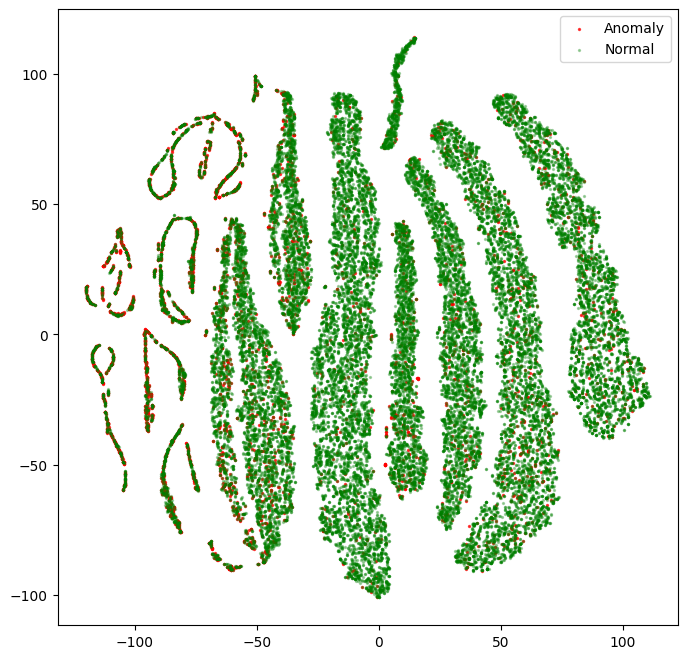
\includegraphics[width=0.75\linewidth]{figures/raw_tsne.png}
    \caption{Two-dimensional t-SNE projection of the input feature space}
    \label{fig:tsne_input}
    \vspace{1mm}
    \begin{minipage}{\columnwidth}
        The projection exhibits class separability between normal and anomalous observations. The plot was obtained using the t-distributed stochastic neighbor embedding (t-SNE) algorithm with two output dimensions and a fixed random seed for reproducibility. The input data was imputed, transformed through bucketing or logarithmic scaling where appropriate, and subsequently encoded for modeling. The scatter plot displays the embedded features color-coded by label, where anomalies (\texttt{y} = 1) are plotted in red and normal samples (\texttt{y} = 0) in green. The embedding was computed using the \texttt{sklearn.manifold} module.
    \end{minipage}
\end{figure}

The t-SNE dimensionality reduction visualization demonstrated in Figure~\ref{fig:tsne_input} reveals that while the majority of anomalies (depicted in red) are dispersed throughout the plot, they tend to cluster near the boundaries of densely populated regions of normal data (in green). This spatial arrangement indicates that anomalous instances are not entirely isolated from the normal data manifold, but instead lie just off its surface. Such a pattern is consistent with the presence of subtle irregularities in the anomalous cases and provides empirical support for the use of reconstruction-based methods, such as autoencoders, for AD, which are designed to model the core structure of normal behavior.

\subsubsection{Preprocessing}

The data preprocessing pipeline consists of the following sequential steps. Imputation was first applied to handle missing values using a combination of mean, median, mode, and domain-specific constants, depending on the distribution and semantic role of each variable. Details about feature-specific imputation rules are shown in \ref{a:data_prep_rule}. In the pre-scaling phase, the variable \texttt{pdays} was bucketed into categorical intervals to account for its non-continuous distribution and the presence of a sentinel value (-1), while log transformations were applied to heavy-tailed variables such as \texttt{duration}, \texttt{campaign}, and \texttt{previous} to reduce skewness. During the encoding step, binary features were mapped to \texttt{0}/\texttt{1}, and categorical variables were converted using one-hot encoding. The dataset was then partitioned into four disjoint subsets: a training set (35\%) consisting solely of normal data for model fitting, a training-validation set (15\%) also limited to normal data for early stopping, a validation set (25\%) containing both normal and anomalous samples for hyperparameter tuning, and a test set (25\%) with labeled data reserved for final evaluation. Table~\ref{tab:data-split} summarizes the size and class composition of each subset. Finally, all numerical features were standardized via normalization followed by \texttt{MinMax} scaling to ensure values lie within the $[0, 1]$ range.

\subfile{tables/data_split}

%%%%%%%%%%%%%%%%%%
%%%%%%%%%%%%%%%%%%
% \begin{figure}[!t]
% 	\centering
% 	\includegraphics[width = \textwidth]{HIS_2_AMZN.png}
% 	\caption{Information Shares for Amazon}
% 	\begin{minipage}{\columnwidth} \footnotesize
% 	\vspace{1mm}
% 	Note: $HIS$ for each interval of AMZN high frequency data sampled every second. Period ranging from 02-01-2020 to 31-01-2020. Each vertical black line represents the start of a new trading day. The information shares are calculated on a 65 minute basis, this results in days being split up in six parts. The mean of all possible orderings of $y_t$ are plotted as well as the upper and lower bounds. The model used is the VECM:
%     \[
%         \Delta y_t = \alpha \beta^\prime y_{t-1} + \sum_{j=1}^{k}\Gamma_{j}\Delta y_{t-j} + \epsilon_t.
%      \]
%      Where $y_t = (MID_t, P_t, WP^{2:5}_t, WP^{6:10}_t)'$. $MID$ represents the mid price, calculated by taking the midpoint of the best BAP. $WP^{n1:n2}$ is the weighted price statistic of the $n1$ to the $n2$ level of the Limit Order Book (LOB). $P$ denotes the most recent transaction price. $k$, the number of lags used in the VECM is selected based on the $AIC$ (Akaike information criterion).
%      \end{minipage}
%      \label{fig:HIS2_AMZN}
% \end{figure}


% As a general guideline, think carefully about your figures and tables and make them in such a way that many results are in there at once: this is good for the overview of the results for the reader.